\section{Study Design}
\label{sec:study-design}
We present the details of our measurement study on bitcoin scam in this section. We first describe our research questions, and then present the dataset used in our study.
\subsection{Research Questions}


\begin{itemize}
    \item[RQ1] \textit{What is the trend of illicit addresses?} We want to measure some basic features of the illicit addresses, including the chronological trends.
    \item[RQ2] \textit{How do the scammers reach victims? What is their behavioral pattern?} We want to identify the behavior of these addresses. For example, how they send out scam messages and make money.
    \item[RQ3] \textit{How much money can these illicit address make?} We want to find out the total amount of money these addresses can get.
    \item[RQ4] \textit{How to detect more illicit addresses based on these addresses?} It is meaningful to find out more addresses based on the collected addresses. This way we can expend our dataset to cover more scam addresses.
    \item[RQ5] \textit{What are the campaign features of these addresses?} It seems that all of the illicit addresses can be categorized into several big campaigns. There are signs that most address belong to certain real-world entity. They deal with the scammed money in an organized way. In solving RQ5 we aim to find out the features of these campaigns.
\end{itemize}

\subsection{Dataset Overview}


We collected our dataset from bitcoinabuse.com, a crowdsourcing public database of bitcoin addresses and other information, used by hackers and criminals\cite{bitcoinabuse}, anyone can file a report on this website. The data collected from this website range from 16th May, 2017 to 18th July, 2020. One example is given in table \ref{table:data_detail}. Abuse type here is provided by the website. The taxonomy is out of the discussion scale in this paper. However, the website provides several tags: ransomware, darknet market, bitcoin tumbler, blackmail scam, sextortion and other (this one can be filled by the users).


\begin{table}

\caption{A Data Example}
\label{table:data_detail}
\begin{tabular}{|l|p{6.5cm}|}

\hline
Address & 1ApsrLsKGwfQeEevLFaVjunNUrNnXSNKGy\\ \hline
Abuse\_type\_id  & blackmail scam \\ \hline
Abuser  & hs3158@mail.edu.tw   \\ \hline
Description & \textit{I run a site in deepweb, I produce all kinds of services in the main it is demolition to business and injury. In general all but murder. Often this happens because of rejected love or competition at business. This month he contacted me and gave me the mission of pour out sourness in your visage. Default order fast, painfully, for life. Without too much fuss. I get money only after finishing task. Thus now I offer you send money to me to be inactive, I propose this to almost all victims. If I do not get money from you, then my performer will fulfill the order. If you transfer me money, besides to my inaction, I will give you info that I have about the customer. After finishing task I always waist the performer, so I have a selection, to get \$1300 from you for info about the customer and my inaction, or to receive \$5000 from the customer, but with a big probability of losing the performer
my BTC address 1ApsrLsKGwfQeEevLFaVjunNUrNnXSNKGy
Two days to decide and pay, and bear in mind that time is ticking.} \\ \hline
From\_country & Mexico\\ \hline
Created\_at & 2019-01-02 23: 22: 06 \\ \hline
\end{tabular}
\end{table}

\begin{figure*}[tbp]
\centerline{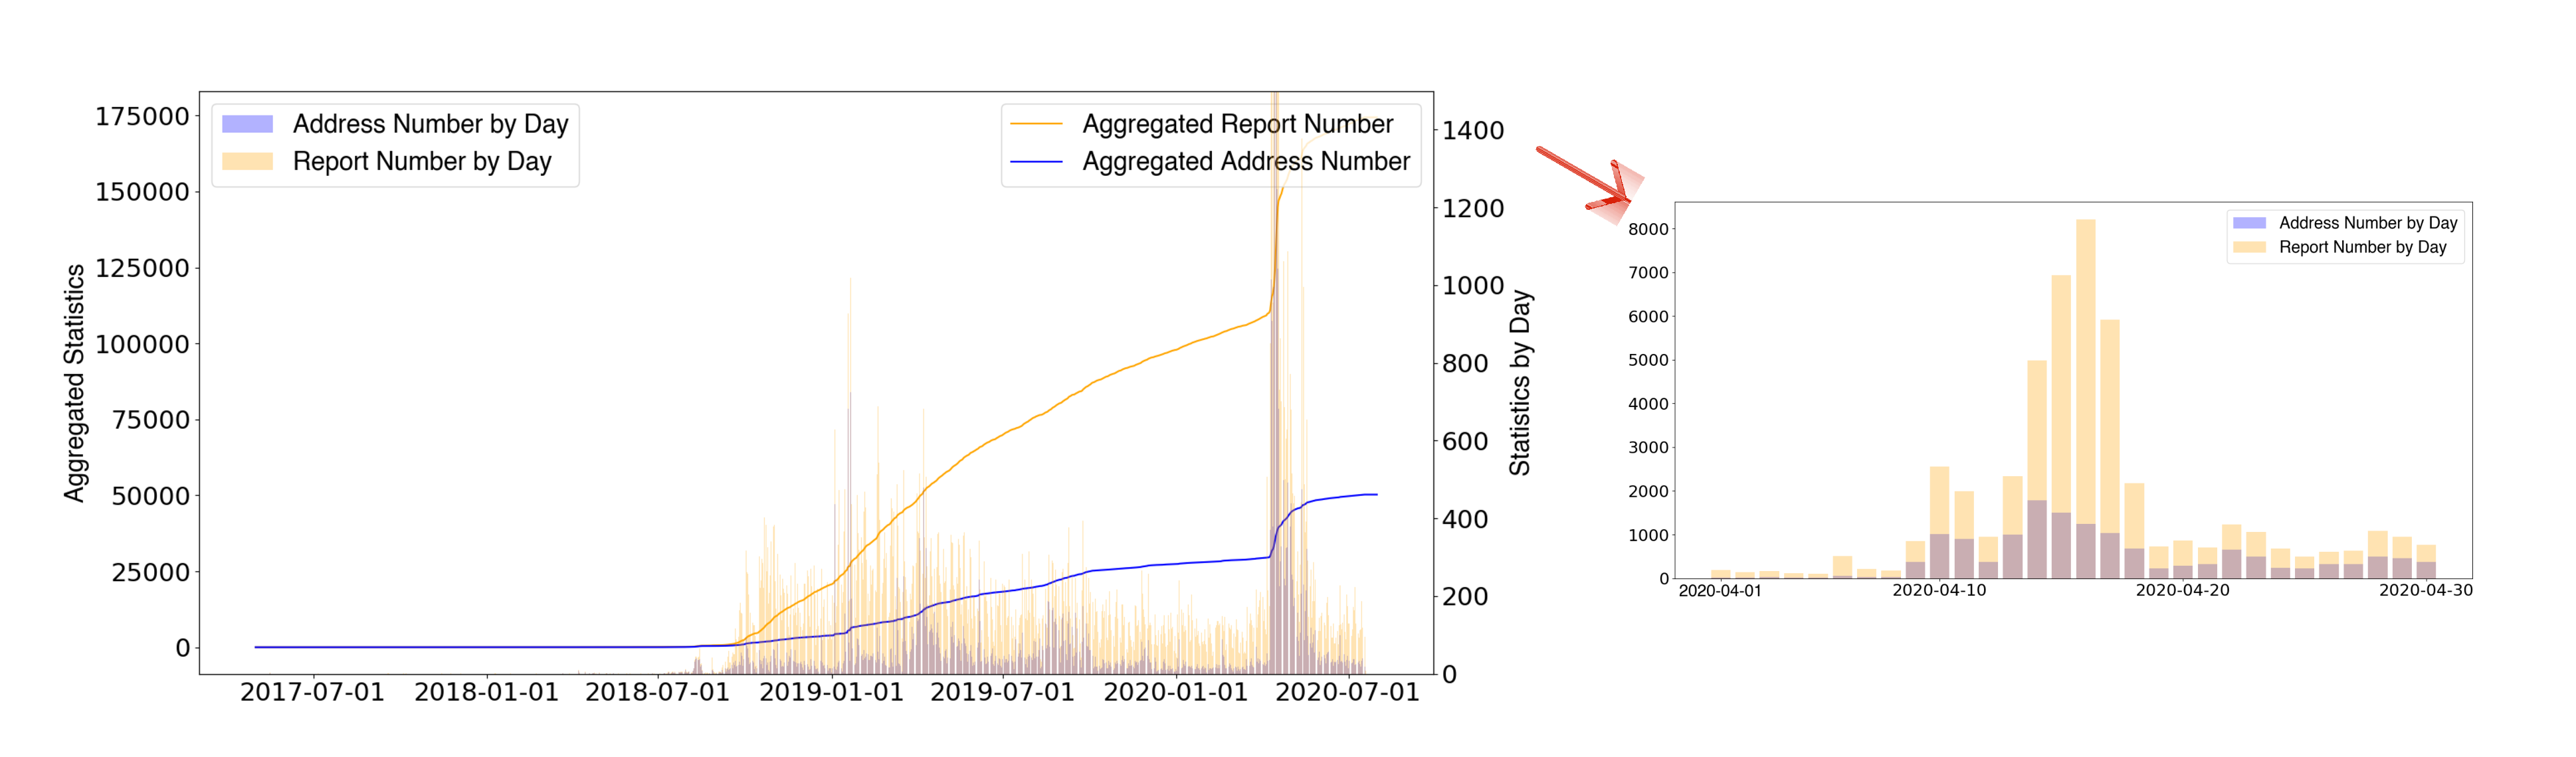
\includegraphics[width=2\columnwidth]{images/full_final_distribution.pdf}}
\caption{The distribution of date in reports.}
\label{fig:date-distribution}
\end{figure*}


Figure \ref{fig:date-distribution} shows the date distribution. The more reports one address gets, the more influence the scam address has in community. In 16th Apr, 2020, the number of reports reached the highest level, with 8,211 reports in a single day. This might be because the beginning of the quarantine period. In other time periods, the report shows a steady growth. This figure also shows the growth of addresses reported.

We also observed that the report comes from different districts around the world. The country distribution is shown in figure  \ref{fig:country-distribution}.

\begin{figure}[tbp]
\centerline{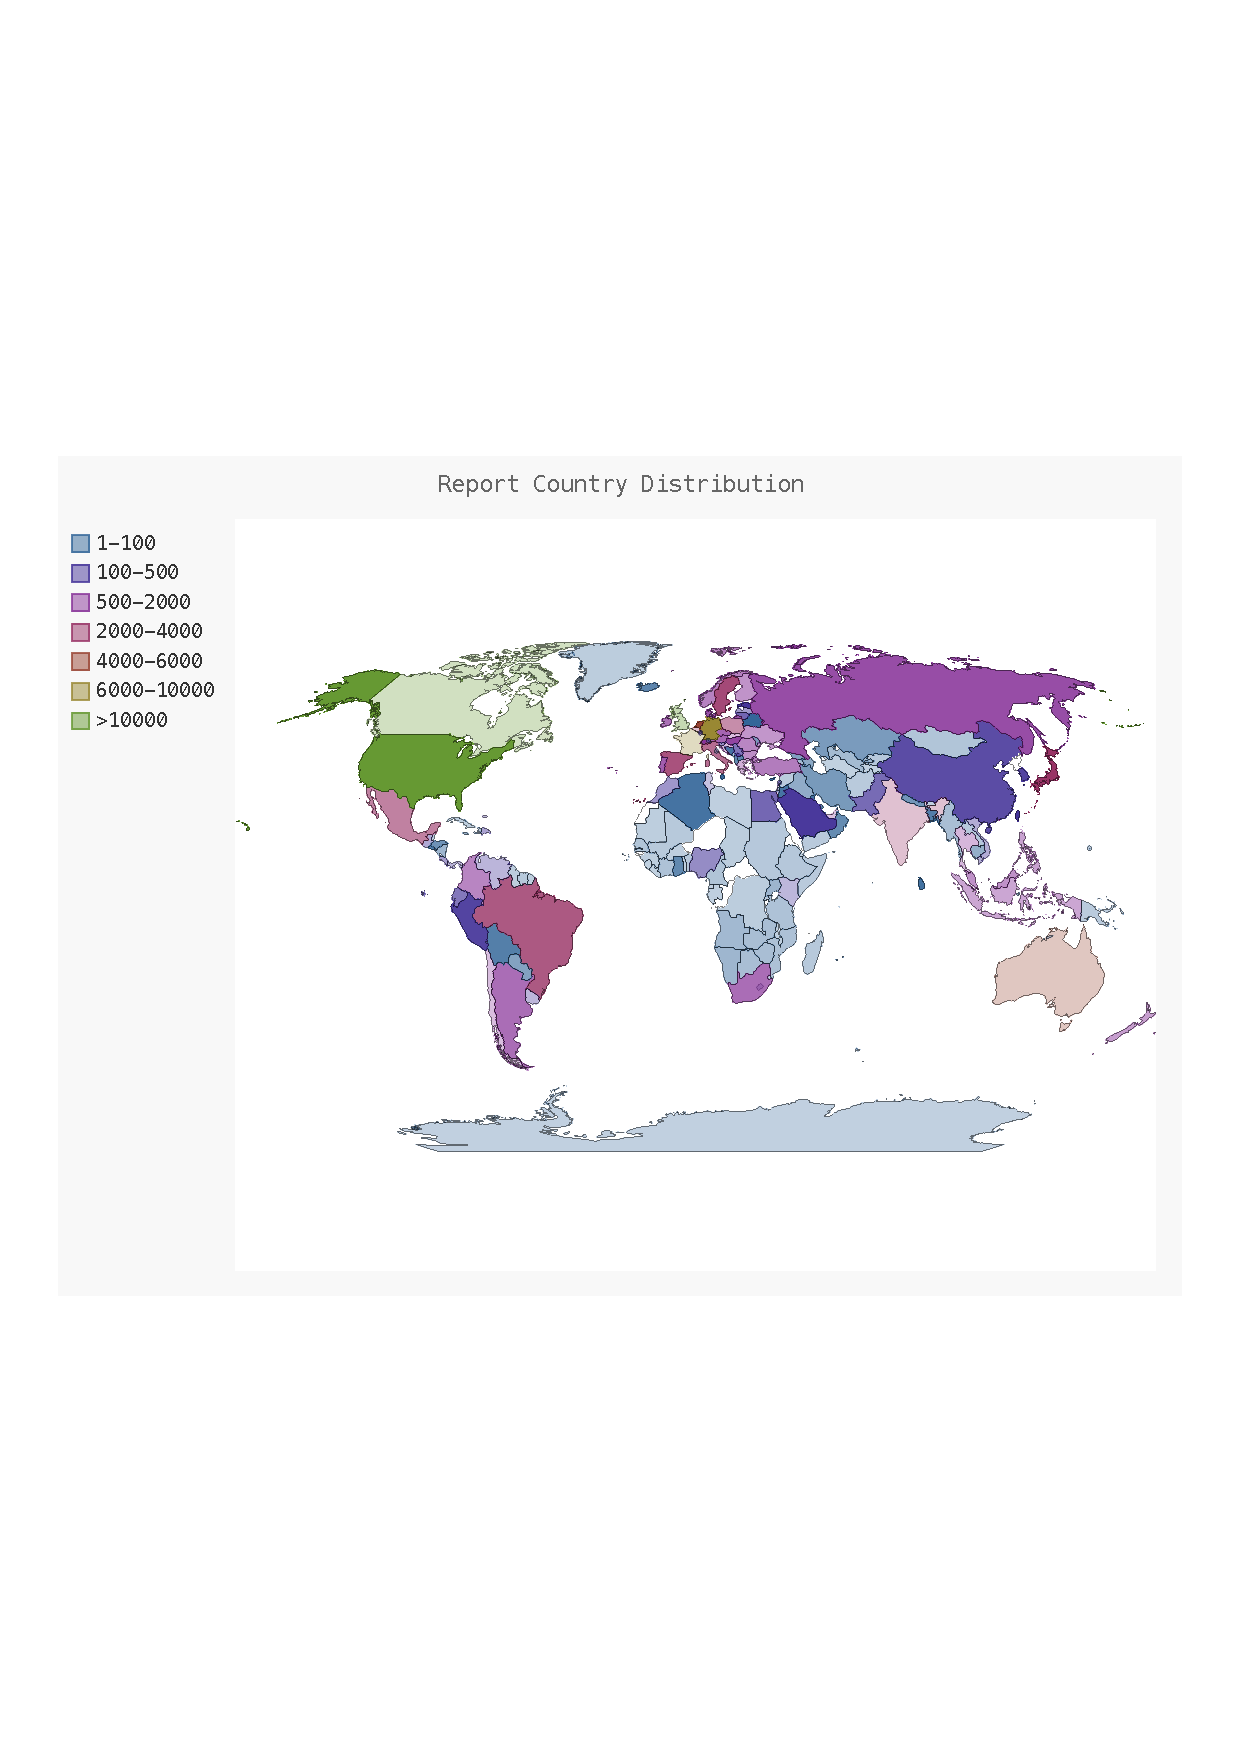
\includegraphics[width=\columnwidth]{images/report_country_distribution.pdf}}
\caption{The time distribution in reports.}
\label{fig:country-distribution}
\end{figure}

After filtering these reports, we got 50,522 unique addresses.




\noindent\fbox{
\begin{minipage}{0.47\textwidth}{
\textbf{Answer to RQ1}: \textit{The reports together with the number of  scam addresses continue to grow, the growth rate came to the peak in April, 2020. One address usually related to multiple reports, the same is for the email addresses.}
}\end{minipage}}






